\documentclass[conference]{IEEEtran}
\IEEEoverridecommandlockouts
\usepackage{amsmath}
% IEEEtran asks for Times as a Type 1 font, which XeTeX (tectonic's engine) cannot load: every bold,
% italic and small-caps shape would silently fall back to upright Latin Modern. So the Times-style
% maths and OpenType text (TeX Gyre Termes) are loaded explicitly.
\usepackage{newtxmath}
\usepackage[no-math]{fontspec}
\setmainfont{texgyretermes}[Extension=.otf, UprightFont=*-regular, BoldFont=*-bold, ItalicFont=*-italic,
  BoldItalicFont=*-bolditalic]
\setsansfont{texgyreheros}[Extension=.otf, UprightFont=*-regular, BoldFont=*-bold, ItalicFont=*-italic,
  BoldItalicFont=*-bolditalic, Scale=MatchLowercase]
\setmonofont{texgyrecursor}[Extension=.otf, UprightFont=*-regular, BoldFont=*-bold, ItalicFont=*-italic,
  BoldItalicFont=*-bolditalic, Scale=MatchLowercase]
\usepackage{booktabs}
\usepackage{array}
\usepackage{graphicx}
\usepackage{tikz}
\usetikzlibrary{positioning,arrows.meta,shapes.misc}
\usepackage{xcolor}
\usepackage[hidelinks]{hyperref}
\usepackage{cite}

% Every number in the results comes from numbers.tex, written by make_figures.py
% from the benchmark's runs (aggregate figures only).
% Written by make_figures.py from runs/. Do not edit by hand.
\newcommand{\NumDocs}{2{,}104}
\newcommand{\NumRenders}{581}
\newcommand{\NumExports}{13}
\newcommand{\NumExportPages}{48}
\newcommand{\NumWorksheets}{44}
\newcommand{\NumHands}{5}
\newcommand{\NumCVLPages}{1{,}604}
\newcommand{\NumMwPages}{150}
\newcommand{\NumRealWriters}{313}
\newcommand{\NumDocConditions}{5{,}304}
\newcommand{\SecondsPerPage}{8}
\newcommand{\SecondsPerScribePage}{3}
\newcommand{\TwinScribeNone}{97.9\%}
\newcommand{\TwinScribeNoneN}{185/189}
\newcommand{\TwinScribeJpeg}{97.4\%}
\newcommand{\TwinScribeJpegN}{184/189}
\newcommand{\TwinScribeDownscale}{91.5\%}
\newcommand{\TwinScribeDownscaleN}{173/189}
\newcommand{\TwinScribePrintscan}{100.0\%}
\newcommand{\TwinScribePrintscanN}{189/189}
\newcommand{\TwinScribePhoto}{98.9\%}
\newcommand{\TwinScribePhotoN}{187/189}
\newcommand{\TwinRealNone}{0.0\%}
\newcommand{\TwinRealNoneN}{0/1765}
\newcommand{\TwinRealJpeg}{0.0\%}
\newcommand{\TwinRealJpegN}{0/561}
\newcommand{\TwinRealDownscale}{0.0\%}
\newcommand{\TwinRealDownscaleN}{0/561}
\newcommand{\TwinRealPrintscan}{0.0\%}
\newcommand{\TwinRealPrintscanN}{0/161}
\newcommand{\TwinRealPhoto}{0.0\%}
\newcommand{\TwinRealPhotoN}{0/561}
\newcommand{\TwinSynthNone}{25.3\%}
\newcommand{\TwinSynthNoneN}{38/150}
\newcommand{\TwinSynthJpeg}{24.7\%}
\newcommand{\TwinSynthJpegN}{37/150}
\newcommand{\TwinSynthDownscale}{19.3\%}
\newcommand{\TwinSynthDownscaleN}{29/150}
\newcommand{\TwinSynthPrintscan}{19.3\%}
\newcommand{\TwinSynthPrintscanN}{29/150}
\newcommand{\TwinSynthPhoto}{11.3\%}
\newcommand{\TwinSynthPhotoN}{17/150}
\newcommand{\TwinRealAllK}{0}
\newcommand{\TwinRealAllN}{3{,}609}
\newcommand{\TwinRealAllUpper}{0.08\%}
\newcommand{\TwinScribeAll}{97.1\%}
\newcommand{\TwinScribeAllN}{918/945}
\newcommand{\TwinScribeCurrent}{100.0\%}
\newcommand{\TwinScribeCurrentN}{612/612}
\newcommand{\TwinScribeOld}{86.1\%}
\newcommand{\TwinScribeOldN}{155/180}
\newcommand{\TwinScribeNew}{99.7\%}
\newcommand{\TwinScribeNewN}{763/765}
\newcommand{\TwinMessMin}{96.3\%}
\newcommand{\TwinMessMax}{99.4\%}
\newcommand{\MessLow}{5}
\newcommand{\MessHigh}{100}
\newcommand{\MessLevels}{6}
\newcommand{\TwinScribeMissK}{27}
\newcommand{\TwinScribeMissOldK}{25}
\newcommand{\TwinScribeMissSuspK}{11}
\newcommand{\TwinScribeSusp}{1.2\%}
\newcommand{\TwinScribeSuspK}{11}
\newcommand{\TwinScribeTooLittle}{0.11\%}
\newcommand{\TwinScribeTooLittleK}{1}
\newcommand{\TwinRealSusp}{0.19\%}
\newcommand{\TwinRealSuspK}{7}
\newcommand{\TwinRealTooLittle}{0.03\%}
\newcommand{\TwinRealTooLittleK}{1}
\newcommand{\TwinSynthSusp}{29.7\%}
\newcommand{\TwinSynthSuspK}{223}
\newcommand{\TwinSynthTooLittle}{0.0\%}
\newcommand{\TwinSynthTooLittleK}{0}
\newcommand{\TwinRealCvlK}{0}
\newcommand{\TwinRealCvlN}{2{,}804}
\newcommand{\TwinRealCvlUpper}{0.11\%}
\newcommand{\TwinRealCvlSusp}{7}
\newcommand{\TwinRealIpadK}{0}
\newcommand{\TwinRealIpadN}{55}
\newcommand{\TwinRealIpadUpper}{5.30\%}
\newcommand{\TwinRealIpadSusp}{0}
\newcommand{\TwinRealMwHumanK}{0}
\newcommand{\TwinRealMwHumanN}{750}
\newcommand{\TwinRealMwHumanUpper}{0.40\%}
\newcommand{\TwinRealMwHumanSusp}{0}
\newcommand{\CnnRandomAuc}{0.975}
\newcommand{\TwinRandomAuc}{0.939}
\newcommand{\CnnRandomFa}{6.9\%}
\newcommand{\TwinRandomFa}{0.0\%}
\newcommand{\CnnRandomDet}{88.9\%}
\newcommand{\TwinRandomDet}{59.7\%}
\newcommand{\RandomDocs}{180}
\newcommand{\RandomTrain}{4{,}935}
\newcommand{\CnnRandomFaNone}{0.9\%}
\newcommand{\TwinRandomFaNone}{0.0\%}
\newcommand{\CnnRandomDetNone}{83.3\%}
\newcommand{\TwinRandomDetNone}{61.1\%}
\newcommand{\CnnRandomFaJpeg}{4.6\%}
\newcommand{\TwinRandomFaJpeg}{0.0\%}
\newcommand{\CnnRandomDetJpeg}{86.1\%}
\newcommand{\TwinRandomDetJpeg}{62.5\%}
\newcommand{\CnnRandomFaDownscale}{0.9\%}
\newcommand{\TwinRandomFaDownscale}{0.0\%}
\newcommand{\CnnRandomDetDownscale}{94.4\%}
\newcommand{\TwinRandomDetDownscale}{55.6\%}
\newcommand{\CnnRandomFaPrintscan}{11.4\%}
\newcommand{\TwinRandomFaPrintscan}{0.0\%}
\newcommand{\CnnRandomDetPrintscan}{88.9\%}
\newcommand{\TwinRandomDetPrintscan}{59.7\%}
\newcommand{\CnnRandomFaPhoto}{19.4\%}
\newcommand{\TwinRandomFaPhoto}{0.0\%}
\newcommand{\CnnRandomDetPhoto}{91.7\%}
\newcommand{\TwinRandomDetPhoto}{59.7\%}
\newcommand{\CnnRandomOnCvl}{0.7\%}
\newcommand{\TwinRandomOnCvl}{0.0\%}
\newcommand{\CnnRandomOnExport}{100.0\%}
\newcommand{\TwinRandomOnExport}{93.3\%}
\newcommand{\CnnRandomOnGenerated}{100.0\%}
\newcommand{\TwinRandomOnGenerated}{97.8\%}
\newcommand{\CnnRandomOnIpad}{0.0\%}
\newcommand{\TwinRandomOnIpad}{0.0\%}
\newcommand{\CnnRandomOnMwHuman}{18.8\%}
\newcommand{\TwinRandomOnMwHuman}{0.0\%}
\newcommand{\CnnRandomOnMwSynthetic}{72.4\%}
\newcommand{\TwinRandomOnMwSynthetic}{4.1\%}
\newcommand{\CnnCleanOnlyAuc}{0.860}
\newcommand{\TwinCleanOnlyAuc}{0.939}
\newcommand{\CnnCleanOnlyFa}{39.8\%}
\newcommand{\TwinCleanOnlyFa}{0.0\%}
\newcommand{\CnnCleanOnlyDet}{93.3\%}
\newcommand{\TwinCleanOnlyDet}{59.7\%}
\newcommand{\CleanOnlyDocs}{180}
\newcommand{\CleanOnlyTrain}{987}
\newcommand{\CnnCleanOnlyFaNone}{1.9\%}
\newcommand{\TwinCleanOnlyFaNone}{0.0\%}
\newcommand{\CnnCleanOnlyDetNone}{69.4\%}
\newcommand{\TwinCleanOnlyDetNone}{61.1\%}
\newcommand{\CnnCleanOnlyFaJpeg}{29.6\%}
\newcommand{\TwinCleanOnlyFaJpeg}{0.0\%}
\newcommand{\CnnCleanOnlyDetJpeg}{100.0\%}
\newcommand{\TwinCleanOnlyDetJpeg}{62.5\%}
\newcommand{\CnnCleanOnlyFaDownscale}{35.2\%}
\newcommand{\TwinCleanOnlyFaDownscale}{0.0\%}
\newcommand{\CnnCleanOnlyDetDownscale}{98.6\%}
\newcommand{\TwinCleanOnlyDetDownscale}{55.6\%}
\newcommand{\CnnCleanOnlyFaPrintscan}{97.1\%}
\newcommand{\TwinCleanOnlyFaPrintscan}{0.0\%}
\newcommand{\CnnCleanOnlyDetPrintscan}{100.0\%}
\newcommand{\TwinCleanOnlyDetPrintscan}{59.7\%}
\newcommand{\CnnCleanOnlyFaPhoto}{74.1\%}
\newcommand{\TwinCleanOnlyFaPhoto}{0.0\%}
\newcommand{\CnnCleanOnlyDetPhoto}{98.6\%}
\newcommand{\TwinCleanOnlyDetPhoto}{59.7\%}
\newcommand{\CnnCleanOnlyOnCvl}{17.1\%}
\newcommand{\TwinCleanOnlyOnCvl}{0.0\%}
\newcommand{\CnnCleanOnlyOnExport}{96.7\%}
\newcommand{\TwinCleanOnlyOnExport}{93.3\%}
\newcommand{\CnnCleanOnlyOnGenerated}{99.5\%}
\newcommand{\TwinCleanOnlyOnGenerated}{97.8\%}
\newcommand{\CnnCleanOnlyOnIpad}{53.3\%}
\newcommand{\TwinCleanOnlyOnIpad}{0.0\%}
\newcommand{\CnnCleanOnlyOnMwHuman}{80.0\%}
\newcommand{\TwinCleanOnlyOnMwHuman}{0.0\%}
\newcommand{\CnnCleanOnlyOnMwSynthetic}{84.8\%}
\newcommand{\TwinCleanOnlyOnMwSynthetic}{4.1\%}
\newcommand{\CnnHoldoutRealCvlAuc}{0.578}
\newcommand{\TwinHoldoutRealCvlAuc}{0.939}
\newcommand{\CnnHoldoutRealCvlFa}{90.9\%}
\newcommand{\TwinHoldoutRealCvlFa}{0.0\%}
\newcommand{\CnnHoldoutRealCvlDet}{70.0\%}
\newcommand{\TwinHoldoutRealCvlDet}{59.7\%}
\newcommand{\HoldoutRealCvlDocs}{472}
\newcommand{\HoldoutRealCvlTrain}{3{,}300}
\newcommand{\CnnHoldoutRealCvlFaNone}{89.8\%}
\newcommand{\TwinHoldoutRealCvlFaNone}{0.0\%}
\newcommand{\CnnHoldoutRealCvlDetNone}{63.9\%}
\newcommand{\TwinHoldoutRealCvlDetNone}{61.1\%}
\newcommand{\CnnHoldoutRealCvlFaJpeg}{93.8\%}
\newcommand{\TwinHoldoutRealCvlFaJpeg}{0.0\%}
\newcommand{\CnnHoldoutRealCvlDetJpeg}{66.7\%}
\newcommand{\TwinHoldoutRealCvlDetJpeg}{62.5\%}
\newcommand{\CnnHoldoutRealCvlFaDownscale}{94.8\%}
\newcommand{\TwinHoldoutRealCvlFaDownscale}{0.0\%}
\newcommand{\CnnHoldoutRealCvlDetDownscale}{68.1\%}
\newcommand{\TwinHoldoutRealCvlDetDownscale}{55.6\%}
\newcommand{\CnnHoldoutRealCvlFaPrintscan}{--}
\newcommand{\TwinHoldoutRealCvlFaPrintscan}{--}
\newcommand{\CnnHoldoutRealCvlDetPrintscan}{69.4\%}
\newcommand{\TwinHoldoutRealCvlDetPrintscan}{59.7\%}
\newcommand{\CnnHoldoutRealCvlFaPhoto}{85.5\%}
\newcommand{\TwinHoldoutRealCvlFaPhoto}{0.0\%}
\newcommand{\CnnHoldoutRealCvlDetPhoto}{81.9\%}
\newcommand{\TwinHoldoutRealCvlDetPhoto}{59.7\%}
\newcommand{\CnnHoldoutRealCvlOnCvl}{90.9\%}
\newcommand{\TwinHoldoutRealCvlOnCvl}{0.0\%}
\newcommand{\CnnHoldoutRealCvlOnExport}{100.0\%}
\newcommand{\TwinHoldoutRealCvlOnExport}{93.3\%}
\newcommand{\CnnHoldoutRealCvlOnGenerated}{100.0\%}
\newcommand{\TwinHoldoutRealCvlOnGenerated}{97.8\%}
\newcommand{\CnnHoldoutRealCvlOnIpad}{0.0\%}
\newcommand{\TwinHoldoutRealCvlOnIpad}{0.0\%}
\newcommand{\CnnHoldoutRealCvlOnMwHuman}{8.8\%}
\newcommand{\TwinHoldoutRealCvlOnMwHuman}{0.0\%}
\newcommand{\CnnHoldoutRealCvlOnMwSynthetic}{25.5\%}
\newcommand{\TwinHoldoutRealCvlOnMwSynthetic}{4.1\%}
\newcommand{\CnnHoldoutRealIpadAuc}{0.599}
\newcommand{\TwinHoldoutRealIpadAuc}{0.936}
\newcommand{\CnnHoldoutRealIpadFa}{94.5\%}
\newcommand{\TwinHoldoutRealIpadFa}{0.0\%}
\newcommand{\CnnHoldoutRealIpadDet}{76.7\%}
\newcommand{\TwinHoldoutRealIpadDet}{59.7\%}
\newcommand{\HoldoutRealIpadDocs}{83}
\newcommand{\HoldoutRealIpadTrain}{4{,}805}
\newcommand{\CnnHoldoutRealIpadFaNone}{100.0\%}
\newcommand{\TwinHoldoutRealIpadFaNone}{0.0\%}
\newcommand{\CnnHoldoutRealIpadDetNone}{73.6\%}
\newcommand{\TwinHoldoutRealIpadDetNone}{61.1\%}
\newcommand{\CnnHoldoutRealIpadFaJpeg}{100.0\%}
\newcommand{\TwinHoldoutRealIpadFaJpeg}{0.0\%}
\newcommand{\CnnHoldoutRealIpadDetJpeg}{72.2\%}
\newcommand{\TwinHoldoutRealIpadDetJpeg}{62.5\%}
\newcommand{\CnnHoldoutRealIpadFaDownscale}{100.0\%}
\newcommand{\TwinHoldoutRealIpadFaDownscale}{0.0\%}
\newcommand{\CnnHoldoutRealIpadDetDownscale}{75.0\%}
\newcommand{\TwinHoldoutRealIpadDetDownscale}{55.6\%}
\newcommand{\CnnHoldoutRealIpadFaPrintscan}{81.8\%}
\newcommand{\TwinHoldoutRealIpadFaPrintscan}{0.0\%}
\newcommand{\CnnHoldoutRealIpadDetPrintscan}{75.0\%}
\newcommand{\TwinHoldoutRealIpadDetPrintscan}{59.7\%}
\newcommand{\CnnHoldoutRealIpadFaPhoto}{90.9\%}
\newcommand{\TwinHoldoutRealIpadFaPhoto}{0.0\%}
\newcommand{\CnnHoldoutRealIpadDetPhoto}{87.5\%}
\newcommand{\TwinHoldoutRealIpadDetPhoto}{59.7\%}
\newcommand{\CnnHoldoutRealIpadOnCvl}{0.0\%}
\newcommand{\TwinHoldoutRealIpadOnCvl}{0.0\%}
\newcommand{\CnnHoldoutRealIpadOnExport}{100.0\%}
\newcommand{\TwinHoldoutRealIpadOnExport}{93.3\%}
\newcommand{\CnnHoldoutRealIpadOnGenerated}{100.0\%}
\newcommand{\TwinHoldoutRealIpadOnGenerated}{97.8\%}
\newcommand{\CnnHoldoutRealIpadOnIpad}{94.5\%}
\newcommand{\TwinHoldoutRealIpadOnIpad}{0.0\%}
\newcommand{\CnnHoldoutRealIpadOnMwHuman}{11.2\%}
\newcommand{\TwinHoldoutRealIpadOnMwHuman}{0.0\%}
\newcommand{\CnnHoldoutRealIpadOnMwSynthetic}{42.1\%}
\newcommand{\TwinHoldoutRealIpadOnMwSynthetic}{4.1\%}
\newcommand{\CnnHoldoutRealMwHumanAuc}{0.397}
\newcommand{\TwinHoldoutRealMwHumanAuc}{0.941}
\newcommand{\CnnHoldoutRealMwHumanFa}{100.0\%}
\newcommand{\TwinHoldoutRealMwHumanFa}{0.0\%}
\newcommand{\CnnHoldoutRealMwHumanDet}{100.0\%}
\newcommand{\TwinHoldoutRealMwHumanDet}{59.7\%}
\newcommand{\HoldoutRealMwHumanDocs}{222}
\newcommand{\HoldoutRealMwHumanTrain}{4{,}345}
\newcommand{\CnnHoldoutRealMwHumanFaNone}{100.0\%}
\newcommand{\TwinHoldoutRealMwHumanFaNone}{0.0\%}
\newcommand{\CnnHoldoutRealMwHumanDetNone}{100.0\%}
\newcommand{\TwinHoldoutRealMwHumanDetNone}{61.1\%}
\newcommand{\CnnHoldoutRealMwHumanFaJpeg}{100.0\%}
\newcommand{\TwinHoldoutRealMwHumanFaJpeg}{0.0\%}
\newcommand{\CnnHoldoutRealMwHumanDetJpeg}{100.0\%}
\newcommand{\TwinHoldoutRealMwHumanDetJpeg}{62.5\%}
\newcommand{\CnnHoldoutRealMwHumanFaDownscale}{100.0\%}
\newcommand{\TwinHoldoutRealMwHumanFaDownscale}{0.0\%}
\newcommand{\CnnHoldoutRealMwHumanDetDownscale}{100.0\%}
\newcommand{\TwinHoldoutRealMwHumanDetDownscale}{55.6\%}
\newcommand{\CnnHoldoutRealMwHumanFaPrintscan}{100.0\%}
\newcommand{\TwinHoldoutRealMwHumanFaPrintscan}{0.0\%}
\newcommand{\CnnHoldoutRealMwHumanDetPrintscan}{100.0\%}
\newcommand{\TwinHoldoutRealMwHumanDetPrintscan}{59.7\%}
\newcommand{\CnnHoldoutRealMwHumanFaPhoto}{100.0\%}
\newcommand{\TwinHoldoutRealMwHumanFaPhoto}{0.0\%}
\newcommand{\CnnHoldoutRealMwHumanDetPhoto}{100.0\%}
\newcommand{\TwinHoldoutRealMwHumanDetPhoto}{59.7\%}
\newcommand{\CnnHoldoutRealMwHumanOnCvl}{0.0\%}
\newcommand{\TwinHoldoutRealMwHumanOnCvl}{0.0\%}
\newcommand{\CnnHoldoutRealMwHumanOnExport}{100.0\%}
\newcommand{\TwinHoldoutRealMwHumanOnExport}{93.3\%}
\newcommand{\CnnHoldoutRealMwHumanOnGenerated}{100.0\%}
\newcommand{\TwinHoldoutRealMwHumanOnGenerated}{97.8\%}
\newcommand{\CnnHoldoutRealMwHumanOnIpad}{0.0\%}
\newcommand{\TwinHoldoutRealMwHumanOnIpad}{0.0\%}
\newcommand{\CnnHoldoutRealMwHumanOnMwHuman}{100.0\%}
\newcommand{\TwinHoldoutRealMwHumanOnMwHuman}{0.0\%}
\newcommand{\CnnHoldoutRealMwHumanOnMwSynthetic}{100.0\%}
\newcommand{\TwinHoldoutRealMwHumanOnMwSynthetic}{4.1\%}
\newcommand{\CnnHoldoutGenScribeAuc}{0.623}
\newcommand{\TwinHoldoutGenScribeAuc}{0.996}
\newcommand{\CnnHoldoutGenScribeFa}{34.3\%}
\newcommand{\TwinHoldoutGenScribeFa}{0.0\%}
\newcommand{\CnnHoldoutGenScribeDet}{2.8\%}
\newcommand{\TwinHoldoutGenScribeDet}{97.1\%}
\newcommand{\HoldoutGenScribeDocs}{297}
\newcommand{\HoldoutGenScribeTrain}{2{,}960}
\newcommand{\CnnHoldoutGenScribeFaNone}{29.6\%}
\newcommand{\TwinHoldoutGenScribeFaNone}{0.0\%}
\newcommand{\CnnHoldoutGenScribeDetNone}{1.1\%}
\newcommand{\TwinHoldoutGenScribeDetNone}{97.9\%}
\newcommand{\CnnHoldoutGenScribeFaJpeg}{29.6\%}
\newcommand{\TwinHoldoutGenScribeFaJpeg}{0.0\%}
\newcommand{\CnnHoldoutGenScribeDetJpeg}{0.0\%}
\newcommand{\TwinHoldoutGenScribeDetJpeg}{97.4\%}
\newcommand{\CnnHoldoutGenScribeFaDownscale}{29.6\%}
\newcommand{\TwinHoldoutGenScribeFaDownscale}{0.0\%}
\newcommand{\CnnHoldoutGenScribeDetDownscale}{0.0\%}
\newcommand{\TwinHoldoutGenScribeDetDownscale}{91.5\%}
\newcommand{\CnnHoldoutGenScribeFaPrintscan}{91.4\%}
\newcommand{\TwinHoldoutGenScribeFaPrintscan}{0.0\%}
\newcommand{\CnnHoldoutGenScribeDetPrintscan}{5.8\%}
\newcommand{\TwinHoldoutGenScribeDetPrintscan}{100.0\%}
\newcommand{\CnnHoldoutGenScribeFaPhoto}{29.6\%}
\newcommand{\TwinHoldoutGenScribeFaPhoto}{0.0\%}
\newcommand{\CnnHoldoutGenScribeDetPhoto}{6.9\%}
\newcommand{\TwinHoldoutGenScribeDetPhoto}{98.9\%}
\newcommand{\CnnHoldoutGenScribeOnCvl}{0.0\%}
\newcommand{\TwinHoldoutGenScribeOnCvl}{0.0\%}
\newcommand{\CnnHoldoutGenScribeOnExport}{9.2\%}
\newcommand{\TwinHoldoutGenScribeOnExport}{90.8\%}
\newcommand{\CnnHoldoutGenScribeOnGenerated}{2.3\%}
\newcommand{\TwinHoldoutGenScribeOnGenerated}{97.6\%}
\newcommand{\CnnHoldoutGenScribeOnIpad}{0.0\%}
\newcommand{\TwinHoldoutGenScribeOnIpad}{0.0\%}
\newcommand{\CnnHoldoutGenScribeOnMwHuman}{100.0\%}
\newcommand{\TwinHoldoutGenScribeOnMwHuman}{0.0\%}
\newcommand{\CnnHoldoutGenMwSyntheticAuc}{0.487}
\newcommand{\TwinHoldoutGenMwSyntheticAuc}{0.912}
\newcommand{\CnnHoldoutGenMwSyntheticFa}{0.4\%}
\newcommand{\TwinHoldoutGenMwSyntheticFa}{0.0\%}
\newcommand{\CnnHoldoutGenMwSyntheticDet}{2.1\%}
\newcommand{\TwinHoldoutGenMwSyntheticDet}{20.0\%}
\newcommand{\HoldoutGenMwSyntheticDocs}{258}
\newcommand{\HoldoutGenMwSyntheticTrain}{4{,}330}
\newcommand{\CnnHoldoutGenMwSyntheticFaNone}{0.0\%}
\newcommand{\TwinHoldoutGenMwSyntheticFaNone}{0.0\%}
\newcommand{\CnnHoldoutGenMwSyntheticDetNone}{0.0\%}
\newcommand{\TwinHoldoutGenMwSyntheticDetNone}{25.3\%}
\newcommand{\CnnHoldoutGenMwSyntheticFaJpeg}{0.0\%}
\newcommand{\TwinHoldoutGenMwSyntheticFaJpeg}{0.0\%}
\newcommand{\CnnHoldoutGenMwSyntheticDetJpeg}{0.0\%}
\newcommand{\TwinHoldoutGenMwSyntheticDetJpeg}{24.7\%}
\newcommand{\CnnHoldoutGenMwSyntheticFaDownscale}{0.0\%}
\newcommand{\TwinHoldoutGenMwSyntheticFaDownscale}{0.0\%}
\newcommand{\CnnHoldoutGenMwSyntheticDetDownscale}{3.3\%}
\newcommand{\TwinHoldoutGenMwSyntheticDetDownscale}{19.3\%}
\newcommand{\CnnHoldoutGenMwSyntheticFaPrintscan}{0.0\%}
\newcommand{\TwinHoldoutGenMwSyntheticFaPrintscan}{0.0\%}
\newcommand{\CnnHoldoutGenMwSyntheticDetPrintscan}{0.7\%}
\newcommand{\TwinHoldoutGenMwSyntheticDetPrintscan}{19.3\%}
\newcommand{\CnnHoldoutGenMwSyntheticFaPhoto}{1.9\%}
\newcommand{\TwinHoldoutGenMwSyntheticFaPhoto}{0.0\%}
\newcommand{\CnnHoldoutGenMwSyntheticDetPhoto}{6.7\%}
\newcommand{\TwinHoldoutGenMwSyntheticDetPhoto}{11.3\%}
\newcommand{\CnnHoldoutGenMwSyntheticOnCvl}{0.7\%}
\newcommand{\TwinHoldoutGenMwSyntheticOnCvl}{0.0\%}
\newcommand{\CnnHoldoutGenMwSyntheticOnIpad}{0.0\%}
\newcommand{\TwinHoldoutGenMwSyntheticOnIpad}{0.0\%}
\newcommand{\CnnHoldoutGenMwSyntheticOnMwHuman}{0.0\%}
\newcommand{\TwinHoldoutGenMwSyntheticOnMwHuman}{0.0\%}
\newcommand{\CnnHoldoutGenMwSyntheticOnMwSynthetic}{2.1\%}
\newcommand{\TwinHoldoutGenMwSyntheticOnMwSynthetic}{20.0\%}
\newcommand{\SensPreSetReal}{0.0\%}
\newcommand{\SensPreSetRealK}{0}
\newcommand{\SensPreSetScribe}{97.1\%}
\newcommand{\SensPreSetScribeK}{918}
\newcommand{\SensPreSetSynthetic}{20.0\%}
\newcommand{\SensPreSetSyntheticK}{150}
\newcommand{\SensMeasuredReal}{0.22\%}
\newcommand{\SensMeasuredRealK}{8}
\newcommand{\SensMeasuredScribe}{98.2\%}
\newcommand{\SensMeasuredScribeK}{928}
\newcommand{\SensMeasuredSynthetic}{37.3\%}
\newcommand{\SensMeasuredSyntheticK}{280}
\newcommand{\SensDsixReal}{0.0\%}
\newcommand{\SensDsixRealK}{0}
\newcommand{\SensDsixScribe}{92.5\%}
\newcommand{\SensDsixScribeK}{874}
\newcommand{\SensDsixSynthetic}{16.8\%}
\newcommand{\SensDsixSyntheticK}{126}
\newcommand{\SensDtenReal}{0.03\%}
\newcommand{\SensDtenRealK}{1}
\newcommand{\SensDtenScribe}{98.7\%}
\newcommand{\SensDtenScribeK}{933}
\newcommand{\SensDtenSynthetic}{22.4\%}
\newcommand{\SensDtenSyntheticK}{168}
\newcommand{\MeasuredRate}{0.13}
\newcommand{\MeasuredRateUpper}{0.16}
\newcommand{\MeasuredLetters}{584{,}523}
\newcommand{\MeasuredCopies}{77}
\newcommand{\MeasuredRateNone}{0.13}
\newcommand{\MeasuredCopiesNone}{77}
\newcommand{\MeasuredLettersNone}{584{,}523}
\newcommand{\MeasuredRateJpeg}{0.21}
\newcommand{\MeasuredCopiesJpeg}{33}
\newcommand{\MeasuredLettersJpeg}{154{,}932}
\newcommand{\MeasuredRateDownscale}{0.06}
\newcommand{\MeasuredCopiesDownscale}{7}
\newcommand{\MeasuredLettersDownscale}{113{,}292}
\newcommand{\MeasuredRatePrintscan}{0.14}
\newcommand{\MeasuredCopiesPrintscan}{2}
\newcommand{\MeasuredLettersPrintscan}{13{,}832}
\newcommand{\MeasuredRatePhoto}{0.08}
\newcommand{\MeasuredCopiesPhoto}{6}
\newcommand{\MeasuredLettersPhoto}{74{,}492}
\newcommand{\MeasuredWorstRate}{0.21}
\newcommand{\MeasuredWorstCondition}{jpeg}
\newcommand{\RealCopyDocs}{46}
\newcommand{\RealDocsNone}{1{,}765}
\newcommand{\RealCopyTopShare}{62\%}
\newcommand{\RealCopyMax}{5}
\newcommand{\RealCopyDispersion}{2.3}
\newcommand{\CopiesCvl}{74}
\newcommand{\LettersCvl}{571{,}812}
\newcommand{\RateCvl}{0.13}
\newcommand{\UpperCvl}{0.16}
\newcommand{\CopiesIpad}{1}
\newcommand{\LettersIpad}{3{,}322}
\newcommand{\RateIpad}{0.30}
\newcommand{\UpperIpad}{1.43}
\newcommand{\CopiesMwHuman}{2}
\newcommand{\LettersMwHuman}{9{,}389}
\newcommand{\RateMwHuman}{0.21}
\newcommand{\UpperMwHuman}{0.67}
\newcommand{\SweepWidths}{3}
\newcommand{\SweepParamsHalf}{0.15~M}
\newcommand{\SweepAucHalf}{0.970}
\newcommand{\SweepCvlHalf}{92.5\%}
\newcommand{\SweepScribeHalf}{4.9\%}
\newcommand{\SweepMinutesHalf}{7}
\newcommand{\SweepParamsOne}{0.58~M}
\newcommand{\SweepAucOne}{0.978}
\newcommand{\SweepCvlOne}{91.5\%}
\newcommand{\SweepScribeOne}{2.8\%}
\newcommand{\SweepMinutesOne}{13}
\newcommand{\SweepParamsTwo}{2.33~M}
\newcommand{\SweepAucTwo}{0.982}
\newcommand{\SweepCvlTwo}{90.3\%}
\newcommand{\SweepScribeTwo}{2.0\%}
\newcommand{\SweepMinutesTwo}{15}
\newcommand{\CvlBeforeFixK}{4}
\newcommand{\CvlBeforeFixN}{1{,}604}
\newcommand{\PrintRecall}{96.7\%}
\newcommand{\PrintFalse}{5.4\%}
\newcommand{\TexAucNone}{0.982}
\newcommand{\TexAucPhoto}{0.857}
\newcommand{\TexHeldCvl}{99.3\%}
\newcommand{\TexHeldIpad}{100.0\%}
\newcommand{\MwExpressions}{4{,}000}
\newcommand{\MwComplex}{18{,}805}
\newcommand{\MwCopies}{0}
\newcommand{\MwRate}{0.00}
\newcommand{\MwUpper}{0.16}
\newcommand{\DistRealTwin}{0.0\%}
\newcommand{\DistRealLetters}{15{,}799}
\newcommand{\DistRealMedian}{0.34}
\newcommand{\DistRealAligned}{41\%}
\newcommand{\DistScribeTwin}{67.8\%}
\newcommand{\DistScribeLetters}{25{,}865}
\newcommand{\DistScribeMedian}{0.04}
\newcommand{\DistScribeAligned}{89\%}
\newcommand{\DistSyntheticTwin}{5.5\%}
\newcommand{\DistSyntheticLetters}{7{,}214}
\newcommand{\DistSyntheticMedian}{0.24}
\newcommand{\DistSyntheticAligned}{25\%}
\newcommand{\DistGeneratedTwin}{73.2\%}
\newcommand{\DistGeneratedLetters}{21{,}218}
\newcommand{\DistGeneratedMedian}{0.04}
\newcommand{\DistGeneratedAligned}{90\%}
\newcommand{\DistExportTwin}{43.1\%}
\newcommand{\DistExportLetters}{4{,}647}
\newcommand{\DistExportMedian}{0.08}
\newcommand{\DistExportAligned}{86\%}
\newcommand{\DistIpadTwin}{0.1\%}
\newcommand{\DistIpadLetters}{2{,}293}
\newcommand{\DistIpadMedian}{0.29}
\newcommand{\DistIpadAligned}{52\%}
\newcommand{\DistCvlTwin}{0.0\%}
\newcommand{\DistCvlLetters}{9{,}674}
\newcommand{\DistCvlMedian}{0.36}
\newcommand{\DistCvlAligned}{49\%}
\newcommand{\DistMwHumanTwin}{0.1\%}
\newcommand{\DistMwHumanLetters}{3{,}832}
\newcommand{\DistMwHumanMedian}{0.31}
\newcommand{\DistMwHumanAligned}{15\%}
\newcommand{\DistMwSyntheticTwin}{5.5\%}
\newcommand{\DistMwSyntheticLetters}{7{,}214}
\newcommand{\DistMwSyntheticMedian}{0.24}
\newcommand{\DistMwSyntheticAligned}{25\%}
\newcommand{\DistDocs}{264}
\newcommand{\DistSetAside}{10{,}958}
\newcommand{\NullRatePerK}{2.0}
\newcommand{\TwinThreshold}{0.08}


\begin{document}

\title{Copies Give It Away: Detecting Sample-Assembled Handwriting by Glyph Reuse, Compared with a Trained Classifier}

\author{\IEEEauthorblockN{Dylan Nguyen}}

\maketitle

\begin{abstract}
Software can now write homework in a student's own handwriting, placing crops of the student's letters, each nudged
by a small random turn, slant or stretch. We test for the trace this leaves: complex letters that coincide with another
letter in the same document once the nudge is undone. The glyph-reuse test aligns each complex letter with its
look-alikes, measures the remaining stroke distance in pen widths, sets printed type and a writer's own copy and paste
aside, and tests the number of near-exact copies against a chance rate for real handwriting. On \NumDocs{} documents
under five conditions, including print-and-scan and phone photographs, it called \TwinScribeAll{} of a commercial
generator's document-conditions generated (\TwinScribeNew{} at its current export resolution) and \TwinRealAllK{} of
\TwinRealAllN{} real-handwriting document-conditions from more than 310 writers. A convolutional network trained on the
same data scores higher within its training distribution (AUC \CnnRandomAuc{} against \TwinRandomAuc{}), but it called
\CnnHoldoutRealCvlFa{} of an unseen real source's documents generated and caught only \CnnHoldoutGenScribeDet{} of an
unseen generator's: it learned where pages came from, not how they were made. Reuse is a narrow signal, blind to
generators that draw every letter afresh and weak against large sample pools, but it holds where the learned detector
breaks, and it shows its evidence.
\end{abstract}

\begin{IEEEkeywords}
handwriting forensics, synthetic handwriting detection, image alignment, generalization, shortcut learning
\end{IEEEkeywords}

% ---------------------------------------------------------------------------
\section{Introduction}

Software can now write homework in a student's own handwriting. It crops the student's letters from a filled
practice sheet and places them, one by one, to spell out a solution, then exports a PDF that looks written by hand.
The result is aimed squarely at a teacher's most basic assumption: that handwriting on a page was put there by a hand.

A detector for such pages can take one of two routes. It can \emph{learn} the difference from labelled examples,
as detectors of synthetic images usually do. Or it can \emph{test} for a trace that the generating process cannot
avoid. For handwriting assembled from samples, that trace is reuse. A person never writes a letter the same way
twice~\cite{srihari2002individuality}. Software that works from one or two samples per character does, nudged each
time by a small turn, slant or stretch. Once that nudge is undone, two copies coincide to within a few hundredths of
a pen width.

This paper builds both detectors and compares them on the same documents. The test-based detector, which we call
the \emph{glyph-reuse test}, needs no examples of any generator; the trained detector is a convolutional network
given every advantage we could give it. Our contributions are:
\begin{itemize}
\item a detector for sample-assembled handwriting that aligns each complex letter with its look-alikes, measures the
  stroke distance that remains, and tests the number of near-exact copies against a chance rate for real handwriting,
  with a stated chance of error and visual evidence a person can check;
\item methods that keep it from mistaking the other exact repeats on real pages for reuse: printed worksheet text
  (by a shape model gated on a smooth page-distortion field) and a writer's own copy and paste;
\item a benchmark of \NumDocs{} documents: exports from a commercial generator, \NumRenders{} pages rendered with its own
  code, real handwriting from \NumRealWriters{} writers on paper and tablets and from MathWriting's contributors, and a
  second, independent generator, each under five conditions including print-and-scan and phone photographs; and
\item a controlled comparison in which a trained classifier beats the test within its training distribution but calls
  most real handwriting from an unseen source generated and misses generators it has not seen, while the test's false
  alarms stay near zero across sources and degradations.
\end{itemize}
The detector, the benchmark and the scripts that produce every number and figure in this paper are
public~\cite{inkcheck}.

% ---------------------------------------------------------------------------
\section{Related Work}

\textbf{Handwriting synthesis.} Neural models generate online handwriting stroke by stroke~\cite{graves2013generating}
and offline word images by adversarial training~\cite{fogel2020scrabblegan}. Such models draw every letter afresh. The
generators studied here instead assemble pages from a writer's own samples, as the consumer application we study does:
it is cheaper, needs no training, and keeps the writer's own letter shapes.

\textbf{Forensic handwriting examination} rests on the individuality of handwriting: no two instances of a letter by
the same writer are identical, while a writer's instances share class characteristics~\cite{srihari2002individuality}.
A traced or copied signature is detected because it superimposes too well on its model. The glyph-reuse test automates
that observation at the scale of every complex letter on a page.

\textbf{Copy-move forgery detection} finds regions of one image that were cloned from another region, by block
matching~\cite{fridrich2003copymove} or by keypoints and a recovered affine transform~\cite{amerini2011sift}. Our setting
differs in scale (letter-sized, not object-sized), in the transforms (a fresh random affine nudge per copy), and in what
else repeats exactly on a genuine page (printed type, pasted ink).

\textbf{Detectors of synthetic images} trained on one generator can transfer to others when trained with broad data and
augmentation~\cite{wang2020cnngenerated}, but deep networks readily learn \emph{shortcuts}: features that separate
training sets without capturing the intended concept~\cite{geirhos2020shortcut}. Section~\ref{sec:generalization} shows
this happening for handwriting.

\textbf{Segmentation.} Cutting handwriting into letters is hard because segmentation and recognition depend on each
other~\cite{sayre1973}. The glyph-reuse test sidesteps recognition: it never asks what a letter is, only whether two
pieces of ink coincide.

% ---------------------------------------------------------------------------
\section{Sample-Assembled Handwriting}
\label{sec:generator}

We study Scribe, a web application that solves an uploaded worksheet with a language model and writes the solution in
the user's handwriting. We read its renderer and export code; this section describes what they do.

\textbf{Samples.} The writer fills a practice sheet with one box per character. Each box is cropped at 2~px per point
(144~dpi) as a mask. In the public hand we examined, 83 of 102 characters have exactly one sample and 19 have two.
Optional sentence pages add a \emph{library} of whole letters and the joins between them, used for prose (496 letter
copies of 29 characters in that hand).

\textbf{Placement.} Each sample is enlarged, re-thresholded to a solid stroke, tinted, and drawn with its own small
change of size (about $\pm5\%$), rotation (about $1.6^\circ$) and slant; lines slope and drift, words vary in size. A
messiness setting from 0 to 100 scales this variation; at 0 each letter keeps half of the default variation. Letters
taken from the library are placed as exact copies (the code calls them ``real copies, never jittered'').

\textbf{Export.} Each page is painted at four times its size in points ($2448\times3168$~px; twice its size before
October 2026), saved as one lossless PNG, and wrapped in a PDF by the pdf-lib library.

Within one document, then, every repeat of a sampled character is the same bitmap under a small affine change, and
library letters repeat with no change at all but the line's slope, much as printed type does. The detector has to
find the first and tell the second from print.

% ---------------------------------------------------------------------------
\section{The Glyph-Reuse Test}
\label{sec:method}

\begin{figure*}[t]
\centering
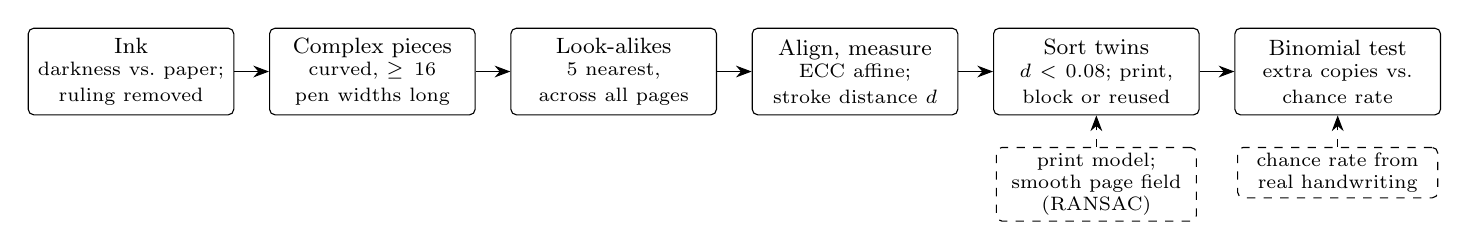
\begin{tikzpicture}[
  node distance=4mm and 4.4mm,
  box/.style={draw, rounded corners=2pt, align=center, font=\footnotesize, inner sep=3pt, minimum height=11mm, text width=24mm},
  side/.style={draw, dashed, rounded corners=2pt, align=center, font=\scriptsize, inner sep=2pt, text width=24mm},
  >={Stealth[length=2mm]}]
\node[box] (ink) {Ink\\{\scriptsize darkness vs.\ paper;\\ruling removed}};
\node[box, right=of ink] (pieces) {Complex pieces\\{\scriptsize curved, $\ge 16$\\pen widths long}};
\node[box, right=of pieces] (cand) {Look-alikes\\{\scriptsize 5 nearest,\\across all pages}};
\node[box, right=of cand] (align) {Align, measure\\{\scriptsize ECC affine;\\stroke distance $d$}};
\node[box, right=of align] (sort) {Sort twins\\{\scriptsize $d<0.08$; print,\\block or reused}};
\node[box, right=of sort] (test) {Binomial test\\{\scriptsize extra copies vs.\\chance rate}};
\node[side, below=of sort] (print) {print model;\\smooth page field\\(RANSAC)};
\node[side, below=of test] (rate) {chance rate from\\real handwriting};
\draw[->] (ink) -- (pieces); \draw[->] (pieces) -- (cand); \draw[->] (cand) -- (align);
\draw[->] (align) -- (sort); \draw[->] (sort) -- (test);
\draw[->, dashed] (print) -- (sort); \draw[->, dashed] (rate) -- (test);
\end{tikzpicture}
\caption{The glyph-reuse test. Only the dashed inputs are learned or measured from data: a model that recognises
printed type, and the rate of near-exact copies on real handwriting. No generated page is used to build the detector.}
\label{fig:pipeline}
\end{figure*}

Fig.~\ref{fig:pipeline} shows the pipeline. Each step is short.

\textbf{Ink.} Darkness is measured against the page's own paper, estimated by a coarse median, so that uneven light
and coloured paper drop out. Ruled and grid lines are removed by subtracting a long, thin morphological opening (a
top-hat), so a letter crossing a line keeps its ink. A hysteresis threshold and connected components cut the ink into
pieces. The pen width $w$ is the ink's area over the length of its centreline, with anti-aliased edge pixels counted by
their share of ink; it matches drawn strokes to within 5\% and sets every scale that follows.

\textbf{Complex pieces.} A dot, a dash, a straight stroke or a ring repeats closely in anyone's hand, so it can never
show reuse. A piece's complexity is its centreline length in pen widths, discounted for straightness:
\begin{equation}
c = \frac{L}{w}\,\min\!\left(1, \max\!\left(0, \frac{\tau - 1}{0.3}\right)\right),
\end{equation}
where $L$ is the centreline length and $\tau = L/\text{(box diagonal)}$ its tortuosity. Pieces with $c < 16$ are
dropped. On real pages, every near-exact twin below that bar was a short, straight stroke.

\textbf{Look-alikes.} Each piece's darkness, stretched to $24\times24$~px and blurred, is a descriptor; its five nearest
descriptors with similar size and aspect, across every page of the document, are candidate twins.

\textbf{Alignment and distance.} Each candidate pair is aligned by maximising the enhanced correlation coefficient
(ECC)~\cite{evangelidis2008ecc}, as implemented in OpenCV~\cite{bradski2000opencv}, under an affine model, coarse to
fine (Gaussian blur of $0.9w$, then $0.35w$); thin strokes are first enlarged to about 3~px. With both aligned pieces
$a$ and $b$ blurred by $w/2$, the remaining root-mean-square stroke distance, in pen widths, is estimated from the
leftover darkness and the darkness gradient, using $b \approx a + \nabla a \cdot u$ for a small displacement field $u$:
\begin{equation}
d = \frac{1}{w}\sqrt{\frac{\sum (a-b)^2}{\tfrac12\sum\left(\lVert\nabla a\rVert^2 + \lVert\nabla b\rVert^2\right)}}.
\end{equation}
Unlike a residual measured in pixels, $d$ does not depend on resolution. Copies of one sample give $d = 0.01$--$0.06$;
a letter written twice by a person gives $0.15$--$0.4$ (Section~\ref{sec:results}). A pair with $d < 0.08$ is a
\emph{twin}.

\textbf{Sorting twins.} Three things repeat exactly on a genuine page besides reused samples, and all three are set aside.

\emph{Printed type.} On a printed or scanned worksheet every copy of a letter in one font is identical. Geometry alone
cannot separate it from library letters, which also repeat rigidly, and a scan adds noise to the turn and size measured
between printed letters (a round letter's rotation is barely defined). A group of twins is therefore set aside as print
when the median of its pieces is judged to be type by a small network: HOG features~\cite{dalal2005hog} and eight size
and stroke measures (stroke-width contrast, endpoints, junctions and the like), one hidden layer of 64 units, trained on letters set in 196 text faces of 64 families (handwriting-style faces
excluded, since text set in one is generated handwriting) against handwriting from generated and real pages. With whole
font families and hands held out it recognises \PrintRecall{} of printed letters and calls \PrintFalse{} of handwritten
letters type. Twins whose shape changes fit one smooth distortion of the page (zero for a flat scan, a gentle gradient
for a photograph, fitted by RANSAC~\cite{fischler1981ransac} per page pair), and whose pieces the model reads as type,
are print too. Lines that are mostly print are print throughout, and a twin that moved rigidly among three or more
printed pieces is print as well: a scan breaks printed letters into fragments, such as the bowl of a g, that the model
cannot read on their own.

\emph{Copied blocks.} Three or more twins moved by one shared map, so that each twin's map sends the others' pieces to
within two pen widths of their partners, are a writer's own copy and paste. Note-taking applications make this common;
blocks are reported but never counted.

\emph{Reused shapes} are every other twin.

\textbf{The test.} Twinned pieces come in pairs, so counting pieces would count a chance coincidence twice. The
statistic is the number of \emph{extra copies}: grouping reused twins into clusters $C$,
\begin{equation}
e = \sum_{C} \left(\lvert C\rvert - 1\right).
\end{equation}
With $n$ complex pieces and $r$ the rate of chance copies in real handwriting, the chance of $e$ or more copies on a
real document is $p = P(X \ge e)$ with $X\sim\mathrm{Binomial}(n, r)$. We fixed $r$ at 2 per 1{,}000 complex letters,
at or above the one-sided 95\% Clopper--Pearson upper bound~\cite{clopper1934} of the rate on the first real pages, before
the larger real sources were collected; Section~\ref{sec:operating} compares it with the rate measured on them. A
document is called \emph{generated} when $e \ge 4$ and $p < 10^{-6}$, and \emph{suspicious} when $p < 0.004$ but the
evidence falls short of that; fewer than 15 complex pieces, or a pen under 0.8~px, is \emph{too little to judge}. The
detector never says a page is human-written.

\textbf{Evidence.} The report shows each group of copies cut from the page, and the closest two laid over each other in
red and blue, black where they agree (Fig.~\ref{fig:evidence}).

\begin{figure}[t]
\centering
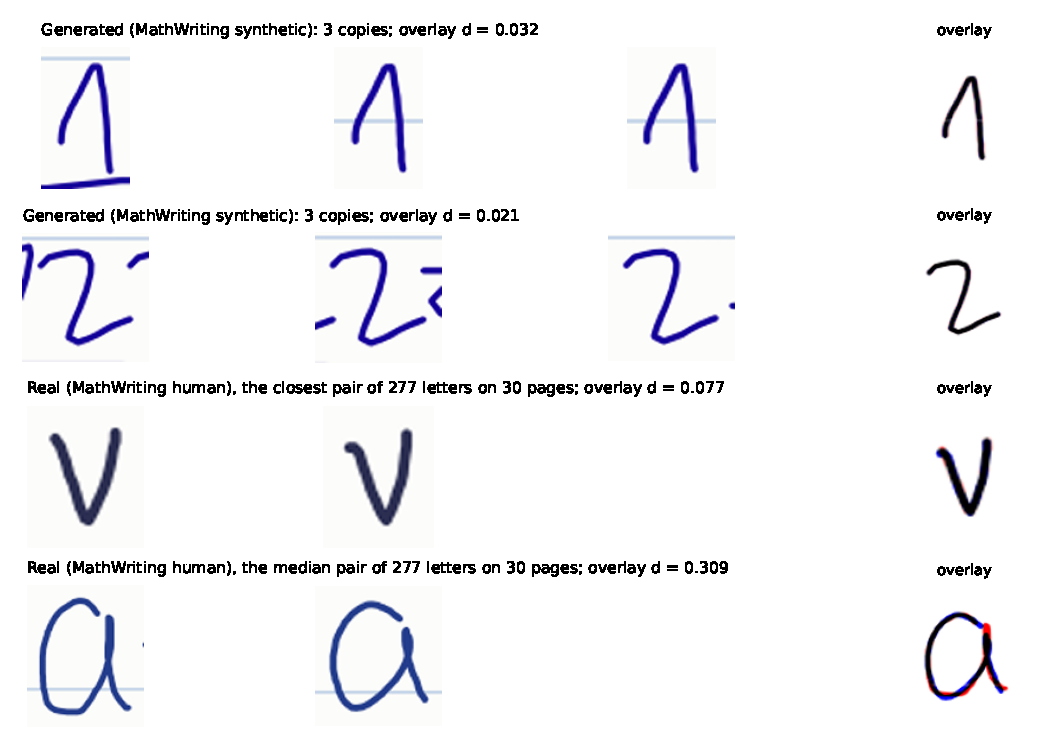
\includegraphics[width=\columnwidth]{figures/evidence.pdf}
\caption{Evidence as the report shows it, on MathWriting pages~\cite{gervais2024mathwriting}. Top two rows: copies of one
glyph on a page from MathWriting's glyph-stitching generator; their overlay is black where the two agree. Bottom two rows:
among 277 complex letters on 30 pages of its contributors' handwriting, the closest pair (two chevron-shaped v's, just
under the twin threshold, which is why one twin is never evidence on its own) and the median pair, whose strokes visibly
part (red and blue).}
\label{fig:evidence}
\end{figure}

\textbf{Other signals.} The file's provenance (which program wrote it, how pages are stored, sensor noise) and a
learned texture score can make a page \emph{suspicious}, never \emph{generated}: metadata is easy to rewrite and
printing erases it, and Section~\ref{sec:generalization} shows why a learned score cannot be trusted further.

% ---------------------------------------------------------------------------
\section{The Trained Baseline}
\label{sec:baseline}

The comparison is a convolutional network that learns ``generated'' against ``real'' from labelled pages, the standard
approach for detecting synthetic images. We gave it every advantage we could.

\textbf{Input.} Pages are normalised exactly as for the glyph-reuse test: darkness against the paper, ruled lines
removed, rescaled so that the pen is 3~px wide. Each page yields 32 patches of $64\times64$~px centred on ink, each
holding a letter or two, so the network learns from ink rather than paper colour or margins.

\textbf{Network.} Seven $3\times3$ convolutions with batch normalisation and ReLU (32 to 256 channels), three max-pooling
layers, global average pooling, dropout of 0.3 and one logistic output: about 0.6 million weights, trained with
AdamW~\cite{loshchilov2019adamw} and a one-cycle schedule for 6 epochs in PyTorch~\cite{paszke2019pytorch}, in about
\SweepMinutesOne{} minutes per model on a laptop GPU.

\textbf{Training data.} Batches are sampled so that each class is half of every batch and each source an equal share of
its class. Every page appears undegraded and under each of the four degradations of Section~\ref{sec:data}, so the
network sees prints, scans and photographs. CVL contributes the same fixed sample of 400 pages that the degraded
benchmark uses.

\textbf{Scoring.} A page's score is the mean of its patches' probabilities, a document's the mean of its pages'; the
decision threshold is 0.5.

We also report a simpler learned model, logistic regression over 44 named features of ink edges (the spread and steps
of edge darkness, edge sharpness, outline detail by frequency band, stroke solidity).

% ---------------------------------------------------------------------------
\section{Data and Protocols}
\label{sec:data}

\begin{table}[t]\centering\caption{Sources. Every document is also evaluated under four degradations.}\label{tab:data}
\footnotesize\setlength{\tabcolsep}{4pt}\begin{tabular}{@{}llrr@{}}\toprule
Source & Truth & Documents & Writers/hands \\\midrule
Scribe, real exports & generated & 13 & 1 writer \\
Scribe, rendered & generated & 176 (581 pp.) & 5 hands \\
MathWriting synthetic & generated & 150 & 6{,}423 glyphs \\
Tablet notes & real & 11 & 3 \\
CVL scans & real & 1{,}604 & 310 \\
MathWriting human & real & 150 & many (mixed) \\
\bottomrule\end{tabular}\end{table}


Table~\ref{tab:data} lists every source.

\textbf{Generated.} \NumExports{} exports were made by a user with the application itself between September and October
2026, across both export resolutions. A further \NumRenders{} pages were rendered with the application's own code, run
unmodified in headless Chrome and verified to match the application's output: \NumWorksheets{} worksheets, each solved by
the application's own solver from a topic prompt, rendered in \NumHands{} hands built from real practice sheets, across
every messiness, paper and ruling setting. A second, independent generator comes from MathWriting~\cite{gervais2024mathwriting},
whose synthetic expressions are stitched together from 6{,}423 individual handwritten glyphs; we set them down in rows,
about fifteen to a page, to make worksheet-like pages.

\textbf{Real.} Real handwriting comes from three sources: pages from a tablet note application by three writers;
\NumCVLPages{} scanned pages from the 310 writers of the CVL database~\cite{kleber2013cvl}, each a printed paragraph
above the writer's handwritten copy of it; and pages of mathematics handwritten on touchscreens by MathWriting's
contributors, set down in the same way as its synthetic expressions. Because MathWriting does not name its writers, its
pages mix writers; Section~\ref{sec:sameWriter} measures same-writer repeats separately, one expression at a time.

\textbf{Degradations.} Each document is evaluated as it is and after JPEG compression (quality 60--85), halving its
resolution, a simulated laser print and 300-dpi scan (toner gain and grain, a slight rotation, scanner blur and noise,
JPEG), and a simulated phone photograph of the printed page (perspective, uneven light and colour cast, blur, sensor
noise, a random resolution, JPEG). Seeds are fixed per document. We call a document under one condition a
\emph{document-condition}. CVL's pages, already scans, are not printed and scanned again, and their other degradations
use a fixed sample of 400 pages.

\textbf{Protocols.} The glyph-reuse test is not trained, so it is simply run on every document. The network is trained
and tested under four protocols, with one model per held-out source:
\begin{enumerate}
\item \emph{random}: documents split 80/20 at random, every source on both sides;
\item \emph{held-out real source}: one real source (CVL, tablet, or MathWriting human) left out of training entirely;
\item \emph{held-out generator}: the application's pages, or the MathWriting generator's, left out of training;
\item \emph{clean only}: trained on undegraded pages, tested under every degradation.
\end{enumerate}
Results for both detectors are reported on exactly the documents each protocol tests.

% ---------------------------------------------------------------------------
\section{Results}
\label{sec:results}

\begin{table*}[t]\centering\caption{Glyph-reuse test: documents called \emph{generated}, by condition. For generated documents this is detection (documents in brackets); for real handwriting it is the false-alarm rate (95\% upper bound in brackets). CVL pages, already scans, are not printed and scanned again, and their other degradations use a fixed sample of 400 pages.}\label{tab:twin}
\footnotesize\begin{tabular}{@{}lrrrrr@{}}\toprule
Documents & As exported & JPEG & Half resolution & Print and scan & Phone photo \\\midrule
Scribe (generated) & 97.9\% (189) & 97.4\% (189) & 91.5\% (189) & 100.0\% (189) & 98.9\% (189) \\
MathWriting synth. (generated) & 25.3\% (150) & 24.7\% (150) & 19.3\% (150) & 19.3\% (150) & 11.3\% (150) \\
Real: tablet & 0/11 [23.8\%] & 0/11 [23.8\%] & 0/11 [23.8\%] & 0/11 [23.8\%] & 0/11 [23.8\%] \\
Real: CVL scans & 0/1{,}604 [0.2\%] & 0/400 [0.7\%] & 0/400 [0.7\%] & -- & 0/400 [0.7\%] \\
Real: MathWriting human & 0/150 [2.0\%] & 0/150 [2.0\%] & 0/150 [2.0\%] & 0/150 [2.0\%] & 0/150 [2.0\%] \\
\bottomrule\end{tabular}\end{table*}

\subsection{The glyph-reuse test}
Table~\ref{tab:twin} gives its verdicts. On real handwriting it called \TwinRealAllK{} of \TwinRealAllN{}
document-conditions generated (one-sided 95\% upper bound \TwinRealAllUpper{}) and \TwinRealSuspK{} suspicious. It
caught \TwinScribeAll{} (\TwinScribeAllN{}) of the commercial generator's document-conditions: \TwinScribeNew{} at
today's export resolution, print-and-scan and photographs included, and \TwinScribeOld{} of those at the half resolution
used before October 2026. Of its \TwinScribeMissK{} misses, \TwinScribeMissOldK{} are those older exports, mostly
with small ruling: their strokes are about a pixel wide, too fine to measure the distance between copies reliably,
above all once the page is halved. \TwinScribeMissSuspK{} of the misses were still marked suspicious. Detection does
not depend on the messiness setting, which scales the very jitter the test undoes: between \TwinMessMin{} and
\TwinMessMax{} of rendered document-conditions were caught at each of the \MessLevels{} settings we rendered, from \MessLow{}
to \MessHigh{}. On one CPU core the test takes a median of \SecondsPerScribePage{}~s per page of the generator's and
\SecondsPerPage{}~s per page over all documents.

\ifdefined\DistDocs
\begin{figure}[t]\centering
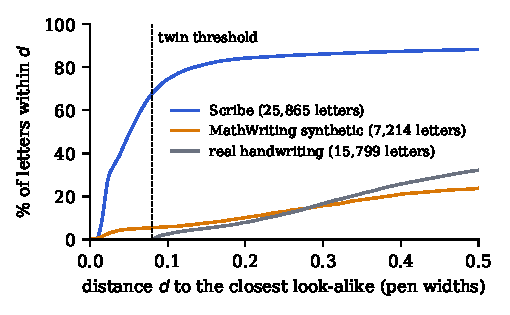
\includegraphics[width=\columnwidth]{figures/distance.pdf}
\caption{The share of complex letters whose closest look-alike in the same document lies within stroke distance $d$, on
\DistDocs{} undegraded documents (up to two pages each). Letters the detector sets aside as printed type or a copied
block are left out. The dashed line is the twin threshold.}\label{fig:distance}
\end{figure}
Fig.~\ref{fig:distance} shows why it works. \DistScribeTwin{} of the commercial generator's complex letters have a twin
closer than the threshold, against \DistRealTwin{} of real letters. Most real letters have no look-alike close enough to
align at all, and those that do lie a median of \DistRealMedian{} pen widths away.
\fi

The second generator is harder. MathWriting's synthetic pages were called generated in \TwinSynthNone{} of cases as
exported, and \TwinSynthSusp{} of its document-conditions were marked suspicious. That generator draws each symbol from
a pool of 6{,}423 glyphs, so a page of fifteen expressions repeats few of them exactly. The power of a reuse test grows
with the length of a document and falls with the number of samples a generator holds per character: one or two per
character, as in the commercial generator, is the easy case; a large pool is not.

\begin{table}[t]\centering\caption{Sensitivity of the operating point (first row): documents called generated when one setting changes. $r$: chance copies per 1{,}000 complex letters; the measured rate is the 95\% upper bound on the 584{,}523 complex letters of the undegraded real documents. $d$: the twin threshold. All conditions pooled: 3{,}609 real, 945 Scribe and 750 MathWriting synthetic document-conditions.}\label{tab:sensitivity}
\footnotesize\begin{tabular}{@{}lrrr@{}}\toprule
Setting & Real & Scribe & MW synth. \\\midrule
$r = 2.00$, $d < 0.08$ (used) & 0 (0.0\%) & 97.1\% & 20.0\% \\
$r = 0.16$ (measured) & 8 (0.22\%) & 98.2\% & 37.3\% \\
$d < 0.06$ & 0 (0.0\%) & 92.5\% & 16.8\% \\
$d < 0.10$ & 1 (0.03\%) & 98.7\% & 22.4\% \\
\bottomrule\end{tabular}\end{table}

\subsection{Operating point}
\label{sec:operating}
Measured on the \MeasuredLetters{} complex letters of the undegraded real documents, the rate of chance copies is
\MeasuredRate{} per 1{,}000 (95\% upper bound \MeasuredRateUpper{}), and no degradation raised it above
\MeasuredWorstRate{}. Most of these copies are printed letters that the rules missed, not handwriting
(Section~\ref{sec:sameWriter}). Table~\ref{tab:sensitivity} changes one setting at a time. The measured bound would
catch more of the second generator (\SensMeasuredSynthetic{} against \SensPreSetSynthetic{}) at the price of more false
alarms (\SensMeasuredRealK{} real document-conditions against \SensPreSetRealK{}). The twin threshold trades the same
way: at $d < 0.06$ the test catches \SensDsixScribe{} of the commercial generator's document-conditions with
\SensDsixRealK{} false alarms, at $d < 0.10$ \SensDtenScribe{} with \SensDtenRealK{}. We keep the pre-set rate. Chance copies are
not independent, as the binomial model assumes: \RealCopyTopShare{} of them sit on 1\% of the real pages, and their
variance across pages is \RealCopyDispersion{} times their mean. A rate an order of magnitude above the measured one
leaves room for that clustering.

\IfFileExists{figures/conditions.pdf}{%
\begin{figure*}[t]\centering
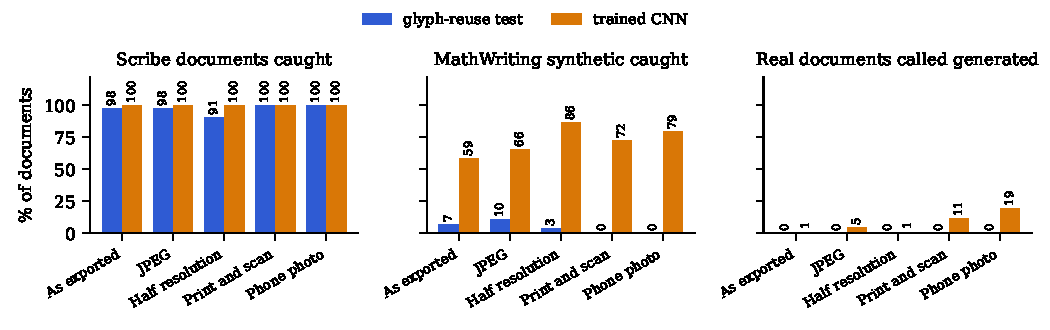
\includegraphics[width=\textwidth]{figures/conditions.pdf}
\caption{Within the network's training distribution (random split; test documents only), by condition. Both detectors
catch nearly all of the commercial generator's documents. The network also learns MathWriting's generator, which the
glyph-reuse test mostly misses, and pays for it in false alarms on degraded real pages.}\label{fig:conditions}
\end{figure*}}{}

\subsection{The trained network, within its distribution}
With every source on both sides of a random split, the network separates generated from real documents with an AUC of
\CnnRandomAuc{} (the test: \TwinRandomAuc{}) and catches \CnnRandomDet{} of generated documents against the test's
\TwinRandomDet{} (Fig.~\ref{fig:conditions}). Both catch nearly all of the commercial generator's documents; the
difference is MathWriting's generator, which the network learns to recognise (\CnnRandomOnMwSynthetic{} caught, against
\TwinRandomOnMwSynthetic{}). It pays in false alarms on degraded real pages: \CnnRandomFaPhoto{} of photographed and
\CnnRandomFaPrintscan{} of printed-and-scanned real documents, against \TwinRandomFaPhoto{} and \TwinRandomFaPrintscan{}
for the test, although every degradation was in its training data. Within its distribution the network is the stronger
detector, but not the more careful one.

% ---------------------------------------------------------------------------
\section{Generalisation}
\label{sec:generalization}

Table~\ref{tab:protocols} and Fig.~\ref{fig:generalization} hold each source out of training in turn.

\IfFileExists{figures/generalization.pdf}{%
\begin{figure*}[t]\centering
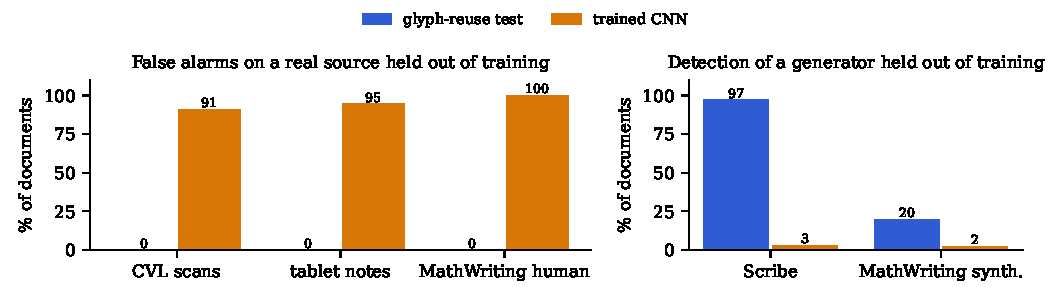
\includegraphics[width=\textwidth]{figures/generalization.pdf}
\caption{Left: real documents called generated when their source was held out of the network's training. Right:
documents caught when their generator was held out. The glyph-reuse test is not trained; it is scored on the same
documents.}\label{fig:generalization}
\end{figure*}}{}

\begin{table*}[t]\centering\caption{The trained CNN against the glyph-reuse test, on the documents each protocol tests (all conditions pooled). False alarms: real documents called generated. Detection: generated documents called generated. A held-out real source's row counts false alarms on that source only; a held-out generator's row counts detection of that generator only. AUC is over the same documents (--: one class only).}\label{tab:protocols}
\footnotesize\begin{tabular}{@{}lrrrrrr@{}}\toprule
 & \multicolumn{2}{c}{AUC} & \multicolumn{2}{c}{False alarms} & \multicolumn{2}{c}{Detection} \\
\cmidrule(lr){2-3}\cmidrule(lr){4-5}\cmidrule(lr){6-7}
Protocol & Twin & CNN & Twin & CNN & Twin & CNN \\\midrule
Random split & 0.939 & 0.975 & 0.0\% & 6.9\% & 59.7\% & 88.9\% \\
Clean-only training & 0.939 & 0.860 & 0.0\% & 39.8\% & 59.7\% & 93.3\% \\
Held-out real: CVL & 0.939 & 0.578 & 0.0\% & 90.9\% & 59.7\% & 70.0\% \\
Held-out real: tablet & 0.936 & 0.599 & 0.0\% & 94.5\% & 59.7\% & 76.7\% \\
Held-out real: MathWriting & 0.941 & 0.397 & 0.0\% & 100.0\% & 59.7\% & 100.0\% \\
Held-out generator: Scribe & 0.996 & 0.623 & 0.0\% & 34.3\% & 97.1\% & 2.8\% \\
Held-out generator: MathWriting & 0.912 & 0.487 & 0.0\% & 0.4\% & 20.0\% & 2.1\% \\
\bottomrule\end{tabular}\end{table*}


\textbf{Unseen real handwriting is called generated.} With CVL held out of training, the network called
\CnnHoldoutRealCvlFa{} of CVL's documents generated; with the tablet pages held out, \CnnHoldoutRealIpadFa{}; with
MathWriting's human pages held out, \CnnHoldoutRealMwHumanFa{}. On the same documents the test called
\TwinHoldoutRealCvlFa{}, \TwinHoldoutRealIpadFa{} and \TwinHoldoutRealMwHumanFa{}. No other threshold would rescue
the network: its AUCs on these documents, \CnnHoldoutRealCvlAuc{}, \CnnHoldoutRealIpadAuc{} and
\CnnHoldoutRealMwHumanAuc{}, are near or below chance.

\textbf{An unseen generator goes undetected.} Trained without the commercial generator's pages, the network caught
\CnnHoldoutGenScribeDet{} of them; trained without MathWriting's generator, \CnnHoldoutGenMwSyntheticDet{} of its pages.
The test caught \TwinHoldoutGenScribeDet{} and \TwinHoldoutGenMwSyntheticDet{} (AUC \TwinHoldoutGenScribeAuc{} and
\TwinHoldoutGenMwSyntheticAuc{}, against the network's \CnnHoldoutGenScribeAuc{} and \CnnHoldoutGenMwSyntheticAuc{}).
Without the commercial generator, the
network also called \CnnHoldoutGenScribeOnMwHuman{} of MathWriting's human pages generated: its only example of
generated handwriting was MathWriting's generator, and what it had learned was the look of MathWriting's pages.

\textbf{Degradation breaks it too.} Trained on undegraded pages only, the network called \CnnCleanOnlyFaPrintscan{} of
printed-and-scanned and \CnnCleanOnlyFaPhoto{} of photographed real documents generated; the test called
\TwinCleanOnlyFaPrintscan{} and \TwinCleanOnlyFaPhoto{} of the same documents.

These are the signatures of shortcut learning~\cite{geirhos2020shortcut}. Each source differs in ways that have nothing
to do with how its handwriting was made: a browser's canvas renders ink in quarter steps of darkness, a scanner blurs and
adds noise, a tablet application draws vector strokes. A network rewarded for separating the training sources learns
those differences first. Faced with a source it has not seen, it files the pages under whichever familiar class they
most resemble. The simpler texture model fails the same way: AUC \TexAucNone{} with writers and hands held out, but
\TexHeldCvl{} of CVL's and \TexHeldIpad{} of the tablet pages called generated once their source was held out.

\begin{table}[t]\centering\caption{Capacity sweep: the network at three widths, each trained and tested as in Table~\ref{tab:protocols}. Random split: AUC. Held-out CVL: CVL documents called generated. Held-out Scribe: Scribe documents caught.}\label{tab:sweep}
\footnotesize\begin{tabular}{@{}lrrr@{}}\toprule
 & Random split & CVL held out & Scribe held out \\
Weights & AUC & false alarms & caught \\\midrule
0.15 M & 0.970 & 92.5\% & 4.9\% \\
0.58 M & 0.978 & 91.5\% & 2.8\% \\
2.33 M & 0.982 & 90.3\% & 2.0\% \\
\bottomrule\end{tabular}\end{table}

\textbf{Capacity is not the cause.} At a quarter and at four times the network's 0.6 million weights (Table~\ref{tab:sweep}), the random split's AUC moves from \SweepAucHalf{} to
\SweepAucTwo{}, but the network still calls \SweepCvlHalf{}, \SweepCvlOne{} and \SweepCvlTwo{} of held-out CVL's
documents generated, and catches \SweepScribeHalf{}, \SweepScribeOne{} and \SweepScribeTwo{} of the held-out
generator's. Size changes how closely the network fits its sources, not what it learns from them.

The glyph-reuse test does not have this failure mode because it never learns what a source looks like. Its only
learned component, the printed-type model, answers a question, ``is this shape type?'', whose training data (196 font
faces) does not depend on any generator.

% ---------------------------------------------------------------------------
\section{Same-Writer Repeats}
\label{sec:sameWriter}

Pages built from MathWriting mix writers, so their twins test whether different people's letters coincide. The
question that matters is whether one person's repeated letters do. Inside a single MathWriting expression every twin is
one writer repeating a symbol. Scored one expression at a time, \MwExpressions{} expressions held \MwComplex{} complex
letters and \MwCopies{} extra copies: \MwRate{} per 1{,}000 (95\% upper bound \MwUpper{}). On the CVL forms, where every
page is also one writer, the rate is \RateCvl{} per 1{,}000 (upper bound \UpperCvl{}), but those copies are almost
all print. We inspected every group of copies on the 43 CVL pages that had any: 48 of the 49 groups were printed type
that the rules had missed (43 bowls of a printed g broken off by the scan, five printed 7s), and one was handwriting,
two cursive l's at $d = 0.072$. Both rates are well under the 2 per 1{,}000 the test assumes. Simple shapes can still
coincide: the closest real pair in Fig.~\ref{fig:evidence}, two chevron-shaped v's, sits just under the threshold. The test tolerates such coincidences by counting them against a chance rate, never treating one
twin as evidence.

% ---------------------------------------------------------------------------
\section{Failure Analysis}
\label{sec:failures}

Every rule in Section~\ref{sec:method} that is not in the basic test was added because a real page was
misjudged. Table~\ref{tab:failures} lists them in the order they were found. We report them because each one is a
way a deployed detector would wrong a student.

\begin{table}[t]\centering
\caption{Misjudgements found while building the detector, and the fix for each.}\label{tab:failures}
\footnotesize
\begin{tabular}{@{}>{\raggedright\arraybackslash}p{0.5\columnwidth}>{\raggedright\arraybackslash}p{0.44\columnwidth}@{}}\toprule
What went wrong & Fix \\\midrule
Real pages: short straight strokes (dashes, 1s) twinned & Complexity discounted for straightness \\
Printed sentences on a real page counted as reuse once a scan removed the PDF's text layer & Twins fitted to one smooth page distortion \\
Repeated printed words looked like copy and paste & Print decided before copied blocks \\
A writer's lasso-copied matrix counted as six reused letters & Copied blocks grouped by a shared map, reported only \\
Library letters (never jittered) set aside as print, 184 of 198 twins on one generated page & Print requires a type-shaped median piece \\
Computer Modern paragraph on every CVL form counted as reuse (8 of 10 sampled pages) & Shape model trained on Computer Modern; print decided per group of twins \\
Binomial test counted both members of each twin, overstating its evidence $10^2$--$10^4$-fold & The statistic counts extra copies \\
Scan-broken fragments of printed letters (the bowl of a g) twinned: \CvlBeforeFixK{} of \CvlBeforeFixN{} CVL pages called generated & Rigid twins among printed pieces are print; some still slip through (Section~\ref{sec:sameWriter}) \\
Old 2$\times$ exports at the smallest ruling missed (letters 12~px tall) & None: a resolution limit; the same worksheet at 4$\times$ is caught \\
\bottomrule
\end{tabular}
\end{table}

Two lessons recur. First, \emph{exact repetition is not evidence by itself}: printed type, a writer's copy and
paste, and a generator's library letters all repeat exactly, and only the combination of how twins move and what they
look like separates them. Second, \emph{measuring every false alarm on real data was the method}: each fix came from a
real page, and synthetic test pages alone would have hidden all of them. An independent code review found the
statistical error, which unit tests on synthetic pages could not have shown.

The same history qualifies our numbers. The real pages that exposed these failures are in the benchmark, so its
false-alarm rates show that the known failures are fixed, not how often unknown ones occur. The last rule, for
scan-broken printed letters, was written after its \CvlBeforeFixK{} CVL pages had been seen.

% ---------------------------------------------------------------------------
\section{Limitations and Ethics}

\textbf{What the test cannot see.} A generator that draws every letter afresh, as neural handwriting
models do~\cite{graves2013generating,fogel2020scrabblegan}, leaves no copies, and neither does one that applies a
different non-rigid distortion to every placement. The glyph-reuse test is blind to both. It is a test for one
mechanism, and makes no claim beyond it.

\textbf{Thin evidence.} A page with few complex letters (one short answer), or strokes under about a pixel wide (an old
low-resolution export shrunk again), cannot be judged, and the detector says so.

\textbf{Real-data coverage.} The rate of chance copies was measured on 310 paper writers, three tablet writers and
MathWriting's contributors, and no real source was held out of the detector's development (Section~\ref{sec:failures}).
Very consistent writers, very small writing or unusual paper may repeat more closely. A source that none of the rules
anticipates, such as a worksheet printed in a typeface unlike any in the print model's training, could produce false
alarms that this benchmark cannot show.

\textbf{One learned baseline.} We trained one family of networks, at three sizes, on patches of ink. Other designs,
such as pretrained backbones, whole-page inputs or a network trained to compare pairs of letters, may generalise
differently, and a learned model of reuse itself is a natural next step. Our claim is narrower: a network trained to
separate generated pages from real ones, as such detectors usually are, learned to tell the sources apart.

\textbf{False accusations.} A detector of academic dishonesty can do harm when wrong. The detector reports evidence
(the copies themselves) rather than a score, never says a page is human-written, and confines every signal that cannot
show its evidence to ``suspicious''. Its verdicts are evidence for a person to weigh, not a judgement about a student.

\textbf{Dual use.} Describing what the test looks for also describes how to evade it. We judged that worth publishing:
the mechanism is simple, its blind spots are stated above, and teachers are better served by knowing both.

\textbf{Data.} The CVL database is licensed for non-commercial research (CC~BY-NC); MathWriting under CC~BY-NC-SA. Real
handwriting from the three tablet writers never leaves the author's machine, and no image of it appears in this paper;
figures show only aggregate numbers and MathWriting's openly licensed ink. The public repository~\cite{inkcheck} holds
code and aggregate results only: CVL and MathWriting must be obtained from their publishers, and neither the tablet
handwriting nor the hands the generator wrote in are released.

% ---------------------------------------------------------------------------
\section{Conclusion}

Handwriting assembled from samples leaves copies, and copies can be found. A test that measures them needs no
examples of any generator, survives printing, scanning and photographs, and shows a person the copies themselves. A
convolutional network trained on the same data was the better detector inside its training distribution and failed
outside it: it called most real pages from an unseen source generated, and missed generators it had not seen.

For a tool whose mistakes fall on students, the second property matters more. The reuse test is narrow: it is blind to
generators that draw every letter afresh, weak against large sample pools, and needs more than a short answer to judge.
Learned detectors will be needed for what reuse cannot see, but they should be judged the way this paper judged
one: on sources, writers and generators held out of training, not on a random split.

\bibliographystyle{IEEEtran}
\bibliography{references}

\end{document}
